\documentclass{article}
\usepackage{geometry}
\geometry{legalpaper, margin=1in}
\usepackage[intlimits]{amsmath}
\usepackage{amsfonts}
\usepackage{amssymb}

\usepackage{dirtytalk}
\usepackage{xcolor}
\usepackage{cancel}

\usepackage{tikz}
\usetikzlibrary{arrows}
\usetikzlibrary{arrows.meta}

\usepackage{xparse}

\definecolor{red}{RGB}{192,22,22}
\definecolor{green}{RGB}{8,140,48}
\definecolor{blue}{RGB}{10,139,200}

\NewDocumentCommand{\parens}{s m}{
    \IfBooleanTF{#1}
    { \ensuremath{ \!\left[ #2 \right] } }
    { \ensuremath{ \!\left( #2 \right) } }
}
\NewDocumentCommand{\Int}{s m o}{
    \int{
        \IfBooleanTF{#1}
        { \ensuremath{ \Bigl[ #2 \Bigr] \IfValueT{#3}{\,\mathrm{d} #3} } }
        { \ensuremath{ #2 \IfValueT{#3}{\,\mathrm{d} #3} } }
    }
}
\NewDocumentCommand{\DInt}{s m m m o}{
    \int\limits_{#2}^{#3}{
        \IfBooleanTF{#1}
        { \ensuremath{ \left[ #4 \right] \IfValueT{#5}{\,\mathrm{d} #5} } }
        { \ensuremath{ #4 \IfValueT{#5}{\,\mathrm{d} #5} } }
    }
}
\NewDocumentCommand{\drv}{s m}{
    \IfBooleanTF{#1}
    { \ensuremath{ \,\mathrm{d} \vec{#2} } }
    { \ensuremath{ \,\mathrm{d} #2 } }
}
\NewDocumentCommand{\ddx}{s D<>{x} o}{
    \IfBooleanTF{#1} { \frac{\partial}{\partial #2} } { \frac{d}{d #2} }
    \IfValueT{#3}{ \ensuremath{ \left[ #3 \right] } }
}
\NewDocumentCommand{\dfdx}{s O{f} O{x}}{
    \IfBooleanTF{#1}
    { \frac{\partial #2}{\partial #3} }
    { \frac{\mathrm{d} #2}{\mathrm{d} #3} }
}

\title{Green's Theorem in Reverse}
\author{OwenTheProgrammer}
\date{\today}

\begin{document}

\maketitle

Green's theorem is often used to convert a line integral problem into an equivalent double integral problem. Green's theorem relates a line integral around a simple closed curve $C$ to a double integral over the planar region $R$ bounded by curve $C$. In some cases though, the double integral is a difficult problem, where an equivalent line integral may prove simple. We will go through the steps to utilize \emph{Green's theorem in reverse} in this short document.

\section{Vector Field Parametrization}

We first define a vector field $\vec{F}$ which returns a force acting upon any given Cartesian coordinate $(x, y)$. $\vec{F}$ returns the force vector with component magnitudes relative to the basis vectors $\hat{i}$ and $\hat{j}$. We will parameterize the actions on each basis vector as separate functions $M$ and $N$, given the $x$ and $y$ coordinates.

\begin{equation}\label{eq:VectorField}
    \vec{F}(x, y) = M(x, y)\hat{i} + N(x, y)\hat{j}
\end{equation}

$M(x, y)$ represents the influence in the $\hat{i}$ direction, while $N(x, y)$ represents the influence in the $\hat{j}$ direction.

\section{Green's Theorem}

Green's theorem is defined as such.

\begin{equation}\label{eq:GreensTheorem}
    \oint_C{ \vec{F} \cdot \drv*{r} }
    = \oint_C{\parens{M \drv{x} + N \drv{y} }}
    = \iint_R{\parens{ \dfdx*[N] - \dfdx*[M][y] }} \drv{A}
\end{equation}

The left integral can be interpreted as the work or \say{effort} done \emph{by} the vector field $\vec{F}$, onto any position $(x, y)$, while taking a infinitesimally small step in direction $\drv*{r}$, along the path $C$.
The \emph{dot product} tracks both the force strength, and how \emph{aligned} the direction $\drv*{r}$ is with the flow of the vector field $\vec{F}$ at position $(x, y)$. This dot product is expanded to the sum of vector components, as shown in the middle integral. The right side re-frames the line integral form as the sum of \emph{circulation densities} or the \emph{k-th component of curl} for region $R$. Curl won't be the guiding topic here, but it's defined as the cross product or \emph{outer product} of a vector fields gradient $\nabla$ in basis $\hat{i}, \hat{j}, \hat{k}$.

\begin{equation}\label{eq:kthCurl}
\begin{aligned}
    \textbf{curl}\:\vec{F}
    &= \nabla\times\vec{F} \\
    &= 
    \parens{\dfdx*[P][y] - \dfdx*[N][z]} \hat{i} -
    \parens{\dfdx*[P][x] - \dfdx*[M][z]} \hat{j} -
    \textcolor{blue}{ \parens{\dfdx*[N][x] - \dfdx*[M][y]} \hat{k} } \\
    \parens{\textbf{curl} \: \vec{F}} \cdot \hat{k}
    &= \dfdx*[N][x] - \dfdx*[M][y]
\end{aligned}
\end{equation}
\emph{The definitions of functions $M$ and $N$ may omit their full signatures for clarity when denoted.}

\section{An Example}
\subsection{Double Integral Method}

Let's execute on an integral that's easy to evaluate for both methods, starting with the traditional double integral method. You may soon notice that this particular example is \emph{much easier} to evaluate through double integration, but \emph{we have different tools for different reasons after all}.

\begin{equation}\label{eq:DoubleIntegralEx1}
    \DInt{1}{2}{\DInt{1}{2}{x^2 + y^2}[y]}[x]
\end{equation}
Since the rules of \emph{Fubini's theorem} apply here, we may solve by \emph{iterated integration} like so.

\begin{equation}
\begin{aligned}
    I &= \DInt*{1}{2}{\DInt{1}{2}{x^2 + y^2}[y]}[x] \\
    &= \DInt*{1}{2}{ \DInt{1}{2}{ \textcolor{blue}{y^0}x^2 + y^2 }[y]}[x] && \text{Introduce hidden constant} \\
    &= \DInt*{1}{2}{ x^2 \DInt{1}{2}{y^0}[y] + \DInt{1}{2}{y^2}[y] }[x] && \text{Separate terms, factor constant} \\
    &= \DInt*{1}{2}{ x^2 \left.\frac{y^1}{1}\right|_1^2 + \left.\frac{y^3}{3}\right|_1^2 }[x] && \text{Power rule for integration} \\
    &= \DInt*{1}{2}{ x^2 \parens*{ 2 - 1} + \parens*{ \frac{2^3}{3} - \frac{1^3}{3} } }[x] && \text{FTC (Part 2)} \\
    &= \DInt*{1}{2}{ x^2 + \frac{7}{3} }[x] \\
    &= \DInt*{1}{2}{ x^2 + \frac{7}{3} \textcolor{blue}{x^0} }[x] && \text{Introduce hidden constant} \\
    &= \DInt{1}{2}{ x^2 }[x] + \frac{7}{3}\DInt{1}{2}{}[x] && \text{Separate terms, factor constant} \\
    &= \left.\frac{x^3}{3}\right|_1^2 + \left.\frac{7x}{3}\right|_1^2 && \text{Power rule for integration} \\
    &= \parens*{\frac{2^3}{3} - \frac{1^3}{3}} + \frac{7}{3}\parens*{2-1} = \frac{7}{3} + \frac{7}{3} = \frac{14}{3}
\end{aligned}
\end{equation}

\begin{equation}\label{eq:DoubleIntegralResult1}
    \DInt{1}{2}{\DInt*{1}{2}{x^2 + y^2}[y]}[x] = \frac{14}{3}
\end{equation}

\subsection{Line Integral Method}

Recall the of the circulation density integral from Green's theorem \eqref{eq:GreensTheorem} and \eqref{eq:kthCurl}. We can restructure this integral to match our original double integral \eqref{eq:DoubleIntegralEx1}. First, let's expand the notation to realize the double integrals are the same but abbreviated.

\begin{equation}
    \iint_R{ \parens{\dfdx*[N][x] - \dfdx*[M][y]} }\drv{A} 
    \to \DInt{a}{b}{\DInt{c}{d}{ \parens{\dfdx*[N][x] - \dfdx*[M][y]} }[y] }[x]
    \quad R \in \parens*{a, b} \times \parens*{c, d}
\end{equation}

To use the relationships proposed in Green's theorem, we must convert our vector field function $\vec{F}$ to an equivalent curl formula \eqref{eq:kthCurl}.

\begin{equation*}
    \parens{ \textbf{curl} \: \vec{F} } \cdot \hat{k} 
    = \dfdx*[N][x] - \dfdx*[M][y] 
    = x^2 + y^2
\end{equation*}

\begin{center}
\noindent\begin{minipage}{0.4\linewidth}
    \begin{equation*}
    \begin{aligned}
        -\dfdx*[M][y] &= y^2 \\
        -\Int{\dfdx*[M][y]}[y] &= \Int{y^2}[y] \\
        -M &= \frac{y^3}{3} \\
        M(x,y) &= -\frac{y^3}{3}
    \end{aligned}
    \end{equation*}
\end{minipage}
\begin{minipage}{0.4\linewidth}
    \begin{equation*}
    \begin{aligned}
        \dfdx*[N][x] &= x^2 \\
        \Int{\dfdx*[N][x]}[x] &= \Int{x^2}[x] \\
        N(x,y) &= \frac{x^3}{3}
    \end{aligned}
    \end{equation*}%
\end{minipage}
\end{center}

We can verify these function choices will work by deriving to undo the work we did. I'd like to note the fact that there is more than one solution for $N$ and $M$, I've just chosen to cancel the partial derivatives through integration.

\begin{equation*}
\begin{aligned}
    M(x, y) = -x^2 y && N(x, y) = y^2 x
\end{aligned}
\end{equation*}
These choices are equally valid, but we will continue nonetheless. We can verify the the new form is correct by computing the derivatives as laid out in their definition.

\begin{equation*}
\begin{aligned}
    \dfdx*[N][x] - \dfdx*[M][y] &= \ddx*[ \frac{x^3}{3} ] - \ddx*<y>[ -\frac{y^3}{3} ] \\
    &= \frac{1}{\cancel{3}}\parens{\cancel{3}x^2} - \frac{1}{\cancel{3}}\parens{-\cancel{3}y^2} \\
    &= x^2 - \parens{-y^2} \\
    &= x^2 + y^2 \\
    \dfdx*[N][x] - \dfdx*[M][y] &= \vec{F}\parens{x, y}
\end{aligned}
\end{equation*}

Now we can comfortably define a line integral with these terms.

\begin{equation}
    \oint_C{\vec{F} \cdot \drv*{r}}
    = \oint_C{\parens{ M \drv{x} + N \drv{y} }}
    = \oint_C{\parens{ \parens*{ -\frac{y^3}{3} } \drv{x} + \parens*{ \frac{x^3}{3}} \drv{y} }}
\end{equation}

\subsubsection{Piecewise Linear Sum}

The diagram in Figure 1 visualizes the bounding segments around region $R$. Technically, the region is defined entirely by curve $C$, but because this region is simple and closed, we can represent the entire curve as a sum of segments. It is \emph{imperative} to evaluate the curve \emph{counter-clockwise}, since the curl vector will face backwards if the direction is reversed.

\begin{center}
    
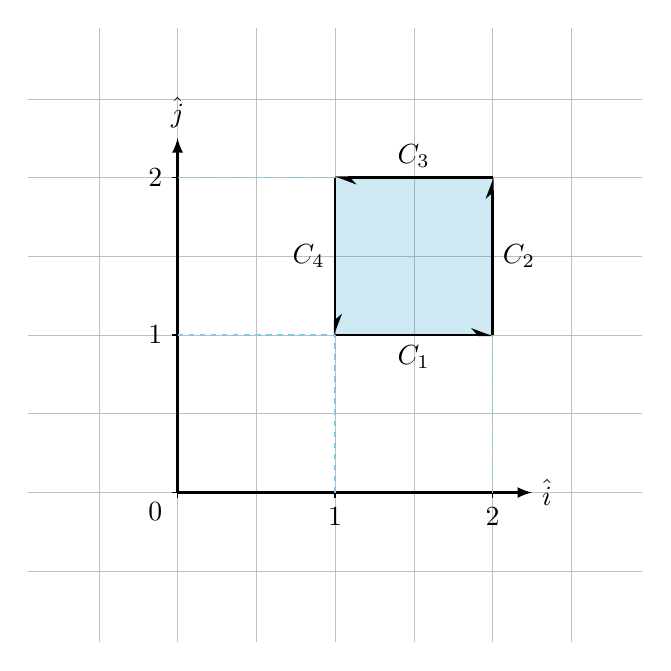
\begin{tikzpicture}
    \tikzstyle{convex_fill}=[thick,-{Stealth[left]}]
    \tikzstyle{bounds}=[-,thin,blue!50,dash pattern=on 2pt off 2pt]
    \coordinate (3) at (2,4); \coordinate (2) at (4,4);
    \coordinate (0) at (2,2); \coordinate (1) at (4,2);
    \draw[step=1cm,gray!50,very thin] (-1.9,-1.9) grid (5.9,5.9);
    \draw[thick,-latex] (0,0) -- (4.5, 0) node[anchor=west] {$\hat{i}$};
    \draw[thick,-latex] (0,0) -- (0, 4.5) node[anchor=south] {$\hat{j}$};
    % Draw the grid markers
    \foreach \x in {1, 2} \draw (\x*2 cm,2pt) -- (\x*2 cm,-2pt) node[anchor=north] {$\x$};
    \foreach \y in {1, 2} \draw (2pt, \y*2 cm) -- (-2pt, \y*2 cm) node[anchor=east] {$\y$};
    \draw (0,2pt) -- (0, -2pt);
    \draw (2pt,0) -- (-2pt, 0) node[anchor=north east] {$0$};
    % Draw the parameter space
    \draw[fill=blue, opacity=0.2] (0) -- (1) -- (2) -- (3) -- cycle;
    \draw[convex_fill] (0) -- (1) node[midway, below] {$C_1$};
    \draw[convex_fill] (1) -- (2) node[midway, right] {$C_2$};
    \draw[convex_fill] (2) -- (3) node[midway, above] {$C_3$};
    \draw[convex_fill] (3) -- (0) node[midway, left] {$C_4$};
    \draw[bounds] (2, 0) -- (0);
    \draw[bounds] (4, 0) -- (1);
    \draw[bounds] (0, 4) -- (3);
    \draw[bounds] (0, 2) -- (0);
\end{tikzpicture}\break
\textsubscript{Figure 1}
\end{center}

Because our region is square in shape, we will have four segments in total. As mentioned beforehand, the sum of those segments will represent the entire curve \emph{en masse}.

\begin{equation}
    \oint_C{\vec{F}\cdot \drv*{r}} = \sum_{i=1}^4{\oint_{C_i}{ \vec{F}\cdot \drv*{r} }}
\end{equation}

To convert our segments to integrable lines, we need to parameterize the domain of each segment $C_n$ as a parametric vector $\vec{r}_n$, dependent on $t$. In essence, we are doing a \emph{change of variables} to make components $x$ and $y$ linearly dependent on $t$. We can also bring the derivatives $dx$ and $dy$ to the $dt$ world. 

We define these vectors based on the endpoints we want for given values $t_0$ and $t_1$ through \emph{linear interpolation}. For example, $C_1$ is a vector constrained by the following.

\begin{equation*}
\begin{aligned}
    \vec{r}_1(t_0) &= (\textcolor{red}{1}, \textcolor{blue}{1}) && \vec{r}_1(t_1) 
    = (\textcolor{red}{2}, \textcolor{blue}{1}) \\
    \vec{r}_1(t=1) &= \textcolor{red}{1\:\hat{i}} + \textcolor{blue}{1\:\hat{j}} &&
    \vec{r}_1(t=2) = \textcolor{red}{2\:\hat{i}} + \textcolor{blue}{1\:\hat{j}} \\
    f_x(t) &= 
    \begin{cases}
        1 & t=1 \\
        2 & t=2
    \end{cases}
    &&
    f_y(t) = \begin{cases}
        1 & t=1 \\
        1 & t=2
    \end{cases} \\
    f_x(t) &= t && f_y(t) = 1 \\
    \vec{r}_1(t) &= t\:\hat{i} + 1\:\hat{j}
\end{aligned}
\end{equation*}

The left section of the following holds each segment $C_n$ as the parameterized vector $\vec{r}_n$, used for the corresponding line integrals on the right.
\begin{center}
\noindent\begin{minipage}{0.4\linewidth}
    \begin{equation*}
    \begin{aligned}
        \vec{r}_1(t) &= t\:\hat{i} + 1\:\hat{j} && t \in \left[1, 2\right] \\
        x &= t && y = 1 \\
        \drv{x} &= 1\drv{t} && \drv{y} = 0\drv{t}
    \end{aligned}
    \end{equation*}
    \begin{equation*}
    \begin{aligned}
        M(x,y) &= \frac{-y^3}{3} \to \frac{-1^3}{3} \\
        N(x,y) &= \frac{x^3}{3} \to \frac{t^3}{3}
    \end{aligned}
    \end{equation*}
\end{minipage}
\begin{minipage}{0.4\linewidth}
    \begin{equation*}
    \begin{aligned}
        C_1 &= \DInt{1}{2}{\parens{ M\drv{x} + N\drv{y} }} \\
        &= \DInt{1}{2}{\parens{ \parens*{\frac{-1^3}{3}} \parens{1\drv{t}} + \cancel{ \parens*{\frac{t^3}{3}} \parens{0\drv{t} } } }} \\
        &= \DInt*{1}{2}{ \frac{-1}{3} }[t] \\
        &= \frac{-1}{3}\DInt{1}{2}{\textcolor{blue}{t^0}}[t]
        = \left.\frac{-t}{3}\right|_1^2
        = \frac{-1}{3}
    \end{aligned}
    \end{equation*}
\end{minipage}
\end{center}

\begin{center}
\noindent\begin{minipage}{0.4\linewidth}
    \begin{equation*}
    \begin{aligned}
        \vec{r}_2(t) &= 2\:\hat{i} + t\:\hat{j} && t \in \left[1, 2\right] \\
        x &= 2 && y = t \\
        \drv{x} &= 0 \drv{t} && \drv{y} = 1 \drv{t}
    \end{aligned}
    \end{equation*}
    \begin{equation*}
    \begin{aligned}
        M(x,y) &= \frac{-y^3}{3} \to \frac{-t^3}{3} \\
        N(x,y) &= \frac{x^3}{3} \to \frac{2^3}{3}
    \end{aligned}
    \end{equation*}
\end{minipage}
\begin{minipage}{0.4\linewidth}
    \begin{equation*}
    \begin{aligned}
        C_2 &= \DInt{1}{2}{\parens{ M \drv{x} + N \drv{y} }} \\
        &= \DInt{1}{2}{\parens{ \cancel{ \parens*{ \frac{-t^3}{3} } \parens{0 \drv{t}} } + \parens*{ \frac{2^3}{3}} \parens{1 \drv{t}} }} \\
        &= \DInt{1}{2}{\parens{ \frac{2^3}{3} }}[t] \\
        &= \frac{8}{3}\DInt{1}{2}{\textcolor{blue}{t^0}}[t]
        = \left.\frac{8t}{3}\right|_1^2
        = \frac{8}{3}
    \end{aligned}
    \end{equation*}
\end{minipage}
\end{center}

\begin{center}
\noindent\begin{minipage}{0.4\linewidth}
    \begin{equation*}
    \begin{aligned}
        \vec{r}_3(t) &= -t\:\hat{i} + 2\:\hat{j} && t \in \left[1, 2\right] \\
        x &= -t && y = 2 \\
        \drv{x} &= -1 \drv{t} && \drv{y} = 0 \drv{t}
    \end{aligned}
    \end{equation*}
    \begin{equation*}
    \begin{aligned}
        M(x, y) &= \frac{-y^3}{3} \to \frac{-2^3}{3} \\
        N(x, y) &= \frac{x^3}{3} \to \frac{-t^3}{3}
    \end{aligned}
    \end{equation*}
\end{minipage}
\begin{minipage}{0.4\linewidth}
    \begin{equation*}
    \begin{aligned}
        C_3 &= \DInt{1}{2}{\parens{ M \drv{x} + N \drv{y} }} \\
        &= \DInt{1}{2}{\parens{ \parens*{\frac{-2^3}{3}} \parens{-1 \drv{t}} + \cancel{ \parens*{\frac{-t^3}{3}} \parens{0 \drv{t}} } }} \\
        &= \DInt{1}{2}{\parens{ \frac{2^3}{3} }}[t] \\
        &= \frac{8}{3}\DInt{1}{2}{\textcolor{blue}{t^0}}[t]
        = \left.\frac{8t}{3}\right|_1^2
        = \frac{8}{3}
    \end{aligned}
    \end{equation*}
\end{minipage}
\end{center}

\begin{center}
\noindent\begin{minipage}{0.4\linewidth}
    \begin{equation*}
    \begin{aligned}
        \vec{r}_4(t) &= 1\:\hat{i} - t\:\hat{j} && t \in \left[1, 2\right] \\
        x &= 1 && y = -t \\
        \drv{x} &= 0 \drv{t} && \drv{y} = -1 \drv{t}
    \end{aligned}
    \end{equation*}
    \begin{equation*}
    \begin{aligned}
        M(x,y) &= \frac{-y^3}{3} \to \frac{t^3}{3} \\
        N(x,y) &= \frac{x^3}{3} \to \frac{1^3}{3}
    \end{aligned}
    \end{equation*}
\end{minipage}
\begin{minipage}{0.4\linewidth}
    \begin{equation*}
    \begin{aligned}
        C_4 &= \DInt{1}{2}{\parens{ M \drv{x} + N \drv{y} }} \\
        &= \DInt{1}{2}{\parens{ \cancel{ \parens*{\frac{t^3}{3}} \parens{0 \drv{t}} } + \parens*{\frac{1^3}{3} \parens{-1\drv{t}}} }} \\
        &= \DInt{1}{2}{\parens{ \frac{-1^3}{3} }}[t] \\
        &= \frac{-1}{3}\DInt{1}{2}{\textcolor{blue}{t^0}}[t]
        = \left.\frac{-t}{3}\right|_1^2
        = \frac{-1}{3}
    \end{aligned}
    \end{equation*}
\end{minipage}
\end{center}

Finally, the sum of all integrated segments work out to be equivalent to the double integral result \eqref{eq:DoubleIntegralResult1}.

\begin{equation}
\begin{aligned}
    \sum_{i=1}^4{\oint_{C_i}{\vec{F} \cdot \drv*{r}}} 
    &= C_1 + C_2 + C_3 + C_4 \\
    &= \frac{-1}{3} + \frac{8}{3} + \frac{8}{3} + \frac{-1}{3} \\
    &= \frac{14}{3}
\end{aligned}
\end{equation}

\end{document}
